\documentclass{article}
\usepackage{amsmath,amssymb,amstext,mathtools,array,url,bm,graphicx,color,epsfig}
\usepackage{fullpage,setspace}
\usepackage{authblk}
\usepackage{filecontents}
\usepackage{natbib}
\usepackage{lineno}
%\usepackage[colorlinks]{hyperref}
\usepackage{hyperref}
\usepackage{subcaption}
\usepackage{float}
\usepackage[flushleft]{threeparttable}

\newtheorem{theorem}{Theorem}
\newtheorem{acknowledgement}[theorem]{Acknowledgement}
\newtheorem{algorithm}[theorem]{Algorithm}
\newtheorem{axiom}[theorem]{Axiom}
\newtheorem{case}[theorem]{Case}
\newtheorem{claim}[theorem]{Claim}
\newtheorem{conclusion}[theorem]{Conclusion}
\newtheorem{condition}[theorem]{Condition}
\newtheorem{conjecture}[theorem]{Conjecture}
\newtheorem{corollary}[theorem]{Corollary}
\newtheorem{criterion}[theorem]{Criterion}
\newtheorem{definition}[theorem]{Definition}
\newtheorem{example}[theorem]{Example}
\newtheorem{exercise}[theorem]{Exercise}
\newtheorem{lemma}[theorem]{Lemma}
\newtheorem{notation}[theorem]{Notation}
\newtheorem{problem}[theorem]{Problem}
\newtheorem{proposition}[theorem]{Proposition}
\newtheorem{remark}[theorem]{Remark}
\newtheorem{solution}[theorem]{Solution}
\newtheorem{summary}[theorem]{Summary}
\newenvironment{proof}[1][Proof]{\noindent\textbf{#1.} }{\ \rule{0.5em}{0.5em}}

\begin{document}
\title{Probability modeling and uncertainty quantification of the Atenquique debris flow, 1955, M\'exico}
\author{}
\maketitle
\abstract
\tableofcontents
\newpage

\section{Introduction}
The hazard assessment of geophysical mass flows commonly relies on the reconstruction of past flows occurred in the area of interest. The available data is commonly related to the properties of the deposit left by the flow, and to the historical documentation. Sometimes it is possible to import data from analog flows occurred elsewhere. In general, this information is affected by relevant sources of uncertainty.

Physical models are adopted to represent the postulated relationship among inputs and outputs of the dynamical system of the mass flow. The choice of the model is a major source of uncertainty, and can lead to inverse problems which are not well-posed. That is, no input data, or not unique input data, are able to produce the observed output.

In this study we detail a new statistical and predictive-oriented procedure, aimed at the hazard assessment of uncertain and poorly constrained geophysical mass flows. We initially set up a uniformly probabilized space $(\Omega_0,\mathcal F, P_0)$ of possible inputs, which we can define arbitrary wide. Then we define a subspace $\Omega\subseteq\Omega_0$ which is obtained under the additional requirement that the simulated flow is numerically stable and reaches a point of interest. If not negligible, this space is naturally measurable with the push-forward of the inclusion $\iota$, normalized to be a probability: 
$$P:=P_0(\Omega)\cdot \iota_*(P_0).$$ 
Then, for each piece of empirical information $D_i$, $i\ge 1$, we define the subspace $\Omega_i\subseteq\Omega$ of the inputs that satisfy it. If not negligible, $\Omega_i$ is probabilized by:
$$P_i:=P(\Omega_i)\cdot \iota^i_*(P),$$
where $\iota^i:\Omega_i\rightarrow \Omega$ is the inclusion function.

The philosophy of our method is based on a sequential application of the empirical falsification principle of Karl R. Popper. In particular, instead of calibrating input data on the empirical information, we use that information to remove those input values which are not consistent with it. Defining the partial solutions subsets $(\Omega_i)_{i\ge1}$ has several advantages compared to a traditionally posed inverse problem: 
\begin{itemize}
  \item the space
  $$\Theta:=\bigcap_i \Omega_i$$ 
  describes the set of the inputs that fully solve the inverse problem; 
  \item the partial solutions $(\Omega_i)_{i\ge1}$ and their intersections can provide information concerning flows that are partially solving the inverse problem, even if $\Theta=\emptyset$;
  \item each probability $P(\Omega_i)$ represents a performance score of the adopted model against the piece of empirical information $D_i$, and can hence be used in model selection framework.
\end{itemize}
We apply our procedure to the case study of the Atenquique volcaniclastic debris flow, occurred in the State of Jalisco (MX), 1955. We adopt and compare the three rheology models \emph{Mohr-Coulomb} (MC), \emph{Pouliquen-Forterre} (PF) and \emph{Voellmy-Salm} (VS).

\section{The Atenquique volcaniclastic debris flow, 1955}

\begin{figure}[H]
\centering
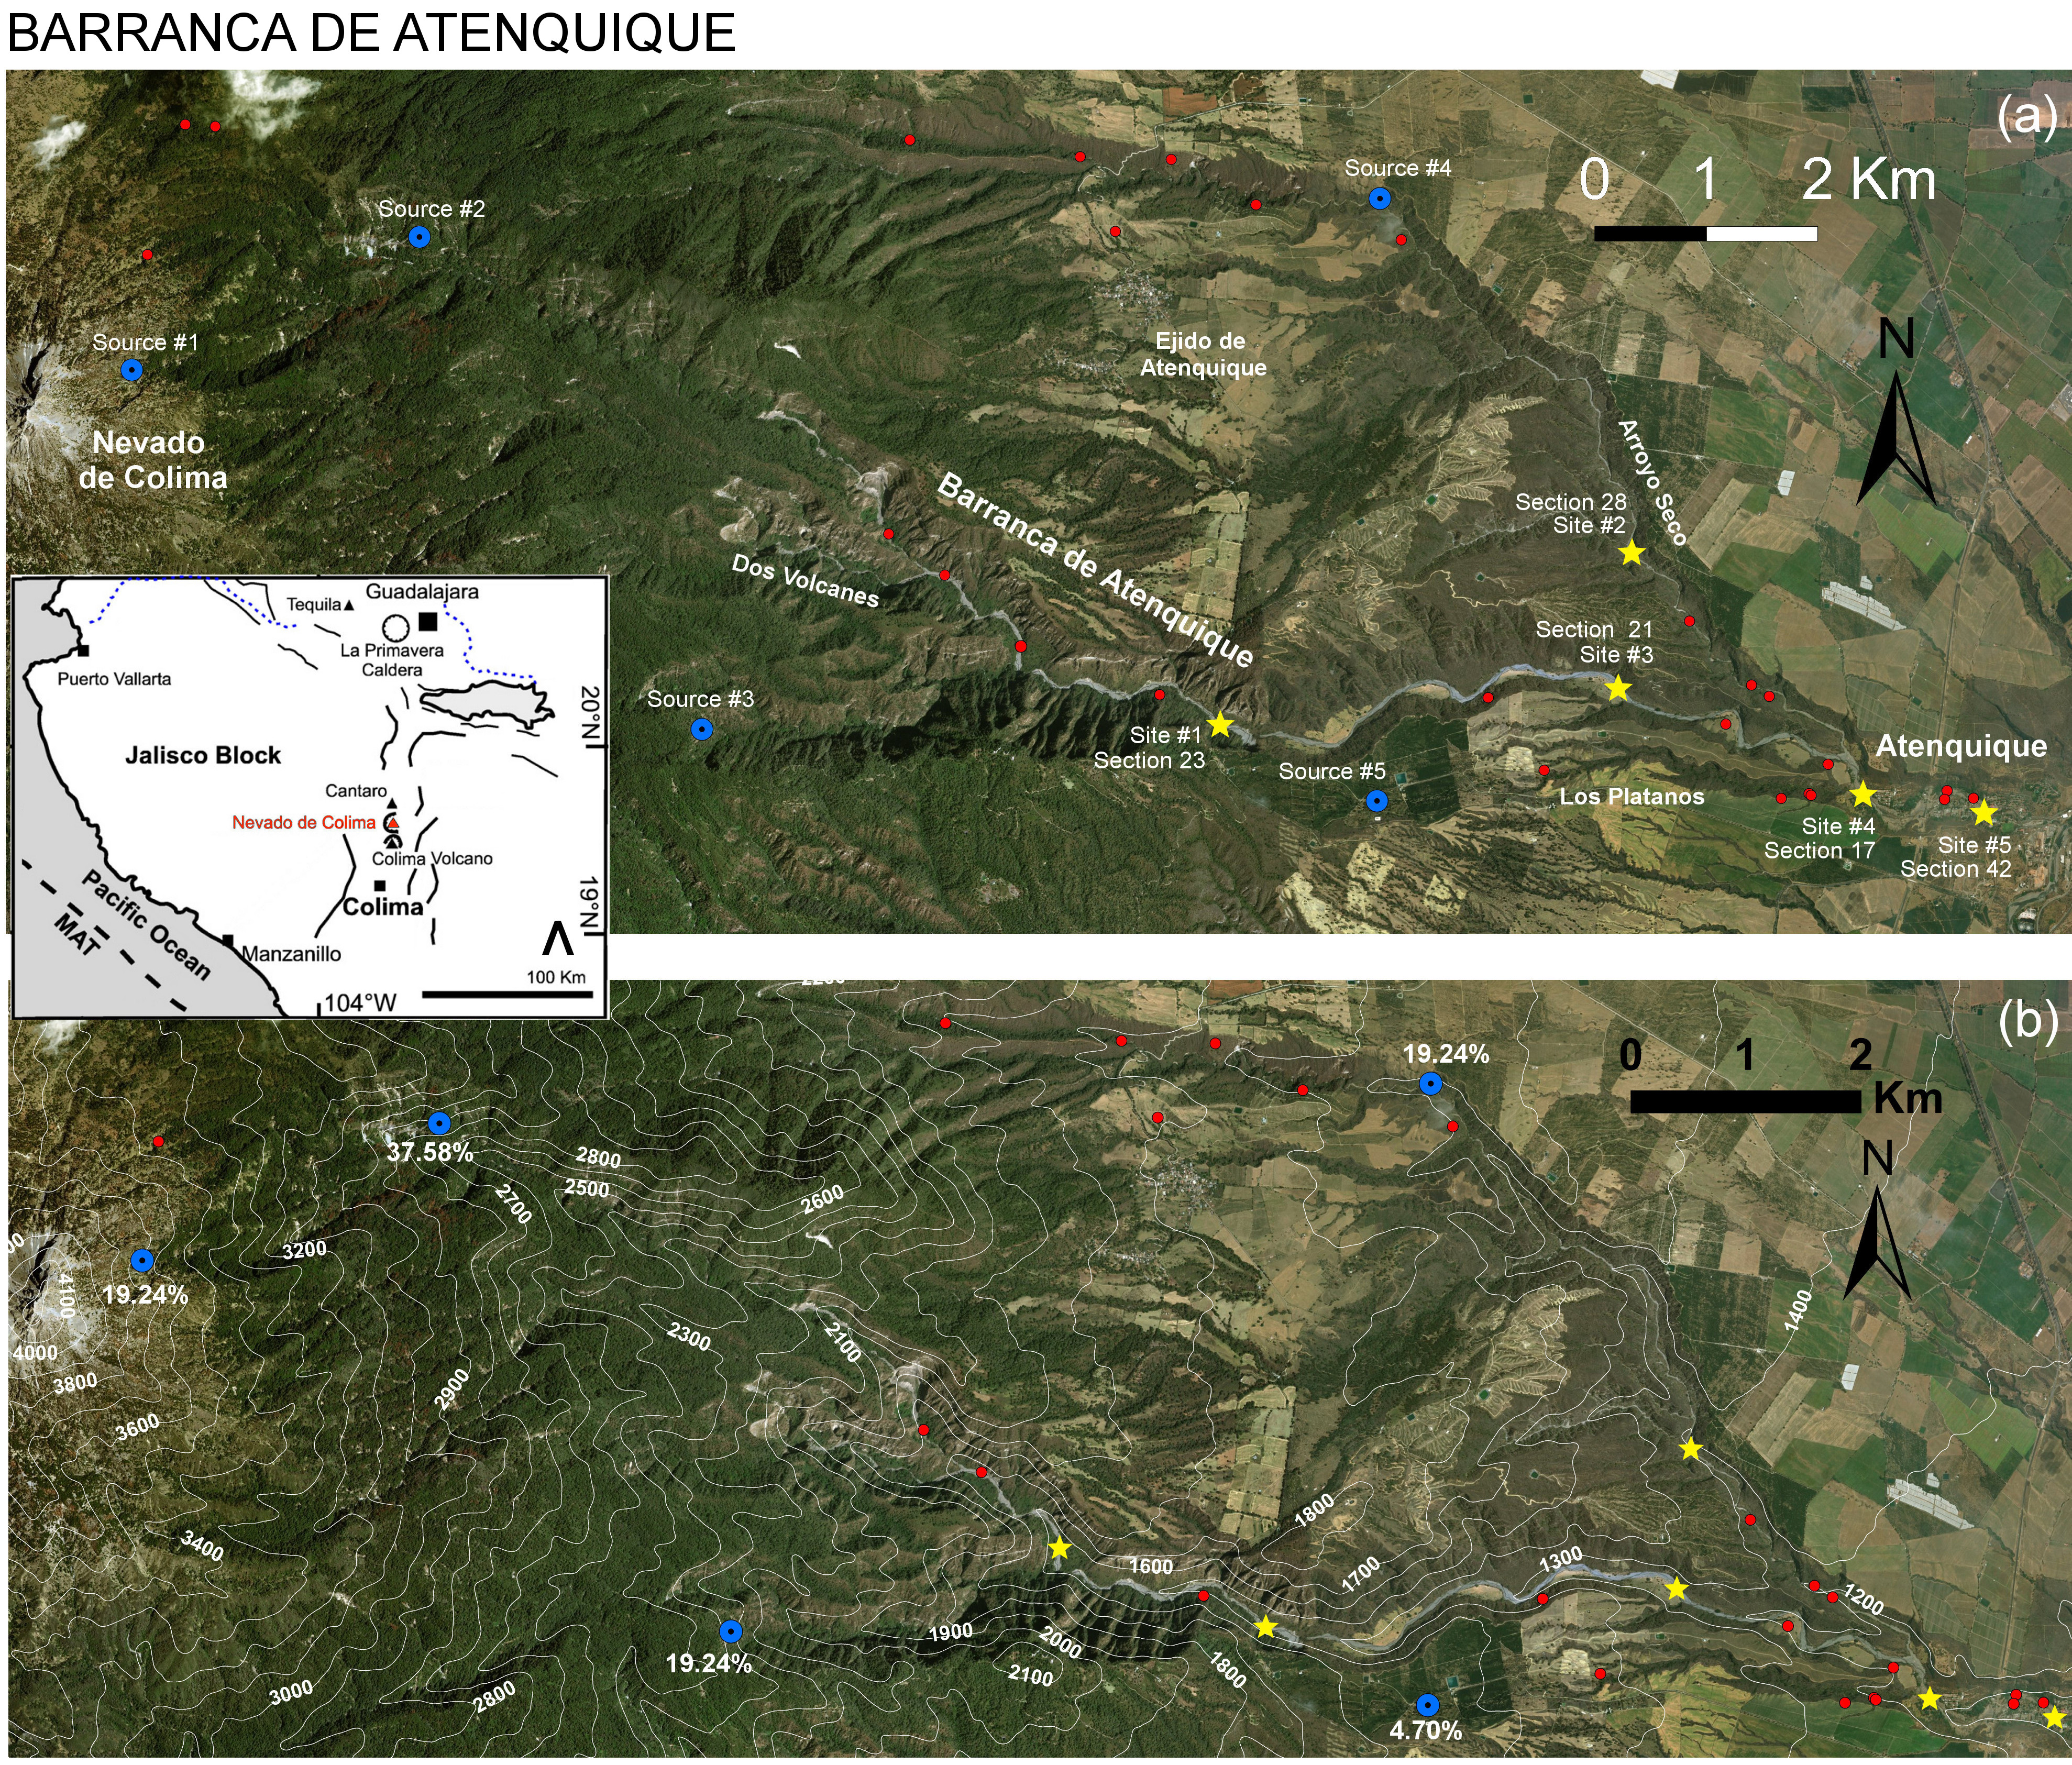
\includegraphics[width=1\textwidth]{Fig1.jpg}
\caption{...}
\label{Fig1}
\end{figure}

\section{Geophysical mass flow models and probability analysis}


\section{Preliminary definition of the input ranges} 

\subsection{Specialized latin hypercube design}
\newpage
\begin{figure}[H]
\centering
\includegraphics[width=0.9\textwidth]{Fig2.png}
\caption{...}
\label{Fig2}
\end{figure}

\subsection{Percentile maps of maximum flow height and kinetic energy}

\begin{figure}[H]
\centering
\includegraphics[width=1\textwidth]{Fig3.png}
\caption{...}
\label{Fig3}
\end{figure}

\begin{figure}[H]
\centering
\includegraphics[width=1\textwidth]{Fig4.png}
\caption{...}
\label{Fig4}
\end{figure}


\section{Observable quantities and contributing variables}

\begin{figure}[H]
\centering
\includegraphics[width=1\textwidth]{Fig5.png}
\caption{...}
\label{Fig5}
\end{figure}

\begin{figure}[H]
\centering
\includegraphics[width=1\textwidth]{Fig6.png}
\caption{...}
\label{Fig6}
\end{figure}

\begin{figure}[H]
\centering
\includegraphics[width=1\textwidth]{Fig7.png}
\caption{...}
\label{Fig7}
\end{figure}

\section{The likelihood of uncertain data}

\begin{figure}[H]
\centering
\includegraphics[width=0.8\textwidth]{Fig8.png}
\caption{...}
\label{Fig8}
\end{figure}

\begin{figure}[H]
\centering
\includegraphics[width=0.8\textwidth]{Fig9.png}
\caption{...}
\label{Fig9}
\end{figure}

\subsection{Alternative performance scores of the models}

\begin{figure}[H]
\centering
\includegraphics[width=1\textwidth]{Fig10.png}
\caption{...}
\label{Fig10}
\end{figure}

\subsection{Conditioning of the specialized latin hypercube design}
\begin{figure}[H]
\centering
\includegraphics[width=0.8\textwidth]{Fig11.png}
\caption{...}
\label{Fig11}
\end{figure}

\subsection{Conditional map of maximum flow height and kinetic energy}

\begin{figure}[H]
\centering
\includegraphics[width=1\textwidth]{Fig12.png}
\caption{...}
\label{Fig12}
\end{figure}

\section*{Acknowledgements}
We would like to acknowledge the support of NSF awards 1521855, 1621853, and 1339765.

\appendix
\section{Pouliquen-Forterre input subspace decomposition}
\begin{figure}[H]
\centering
\includegraphics[width=0.8\textwidth]{FigA1.png}
\caption{...}
\label{FigA1}
\end{figure}

\begin{figure}[H]
\centering
\includegraphics[width=0.8\textwidth]{FigA2.png}
\caption{...}
\label{FigA2}
\end{figure}

\bibliographystyle{apalike}
\bibliography{mybibfileMX}
\end{document}

